\documentclass[letterpaper,12pt,oneside]{article}\usepackage[]{graphicx}\usepackage[]{color}
%% maxwidth is the original width if it is less than linewidth
%% otherwise use linewidth (to make sure the graphics do not exceed the margin)
\makeatletter
\def\maxwidth{ %
  \ifdim\Gin@nat@width>\linewidth
    \linewidth
  \else
    \Gin@nat@width
  \fi
}
\makeatother

\definecolor{fgcolor}{rgb}{0.345, 0.345, 0.345}
\newcommand{\hlnum}[1]{\textcolor[rgb]{0.686,0.059,0.569}{#1}}%
\newcommand{\hlstr}[1]{\textcolor[rgb]{0.192,0.494,0.8}{#1}}%
\newcommand{\hlcom}[1]{\textcolor[rgb]{0.678,0.584,0.686}{\textit{#1}}}%
\newcommand{\hlopt}[1]{\textcolor[rgb]{0,0,0}{#1}}%
\newcommand{\hlstd}[1]{\textcolor[rgb]{0.345,0.345,0.345}{#1}}%
\newcommand{\hlkwa}[1]{\textcolor[rgb]{0.161,0.373,0.58}{\textbf{#1}}}%
\newcommand{\hlkwb}[1]{\textcolor[rgb]{0.69,0.353,0.396}{#1}}%
\newcommand{\hlkwc}[1]{\textcolor[rgb]{0.333,0.667,0.333}{#1}}%
\newcommand{\hlkwd}[1]{\textcolor[rgb]{0.737,0.353,0.396}{\textbf{#1}}}%

\usepackage{framed}
\makeatletter
\newenvironment{kframe}{%
 \def\at@end@of@kframe{}%
 \ifinner\ifhmode%
  \def\at@end@of@kframe{\end{minipage}}%
  \begin{minipage}{\columnwidth}%
 \fi\fi%
 \def\FrameCommand##1{\hskip\@totalleftmargin \hskip-\fboxsep
 \colorbox{shadecolor}{##1}\hskip-\fboxsep
     % There is no \\@totalrightmargin, so:
     \hskip-\linewidth \hskip-\@totalleftmargin \hskip\columnwidth}%
 \MakeFramed {\advance\hsize-\width
   \@totalleftmargin\z@ \linewidth\hsize
   \@setminipage}}%
 {\par\unskip\endMakeFramed%
 \at@end@of@kframe}
\makeatother

\definecolor{shadecolor}{rgb}{.97, .97, .97}
\definecolor{messagecolor}{rgb}{0, 0, 0}
\definecolor{warningcolor}{rgb}{1, 0, 1}
\definecolor{errorcolor}{rgb}{1, 0, 0}
\newenvironment{knitrout}{}{} % an empty environment to be redefined in TeX

\usepackage{alltt}
\usepackage[paperwidth=8.5in,paperheight=11in,top=1in,bottom=1in,left=1in,right=1in]{geometry}
\usepackage{setspace}
\usepackage[colorlinks=true,allcolors=Blue]{hyperref}
\usepackage[usenames,dvipsnames]{xcolor}
\usepackage{indentfirst}
\usepackage{titlesec}
\usepackage{multirow}
\usepackage{booktabs}
\usepackage{graphicx}
\usepackage{verbatim}
\usepackage{rotating}
\usepackage{tabularx}
\usepackage{outlines}
\usepackage{lineno}
\usepackage{array}
\usepackage{times}
\usepackage{cleveref}
\usepackage{acronym}
\usepackage[position=t]{subfig}
\usepackage{paralist}
\usepackage[noae]{Sweave}
\usepackage{natbib}
\usepackage{array}
\usepackage{pdflscape}
\usepackage{bm}
\usepackage{fixltx2e}
% \usepackage{showlabels}
\bibpunct{(}{)}{,}{a}{}{,}

% page margins and section title formatting
\linespread{1.5}
\setlength{\footskip}{0.5in}
\titleformat*{\section}{\Large\bf\em}
\titleformat*{\subsection}{\singlespace\large\bf}
\titleformat*{\subsubsection}{\singlespace\normalsize\bf\em}
\titlespacing{\section}{0in}{0in}{0in}
\titlespacing{\subsection}{0in}{0in}{0in}
\titlespacing{\subsubsection}{0in}{0in}{0in}

% cleveref options
\crefname{table}{Table}{Tables}
\crefname{figure}{Fig.}{Figs.}
\renewcommand{\figurename}{Fig.}

% aliased citations
\defcitealias{LehrterIR}{Lehrter et al. in review}

%acronyms
\acrodef{chla}[chl-\textit{a}]{chlorophyll \textit{a}}
\acrodef{cgem}[CGEM]{Coastal General Ecosystem Model}
\acrodef{do}[O$_2$]{dissolved oxygen}
\acrodef{gom}[GOM]{Gulf of Mexico}
\acrodef{lcs}[LCS]{Louisiana continental shelf}
\acrodef{marb}[MARB]{Mississippi-Atchafalaya River Basin}
\acrodef{oned}[1-D]{one-dimensional}
\acrodef{par}[PAR]{photosynthetically active radiation}

%for supplemental figures/tables
\newcommand{\beginsupplement}{%
        \setcounter{table}{0}
        \renewcommand{\thetable}{S\arabic{table}}%
        \setcounter{figure}{0}
        \renewcommand{\thefigure}{S\arabic{figure}}%
     }

%knitr options


% get the version based on commit date


% get online bib file


\IfFileExists{upquote.sty}{\usepackage{upquote}}{}
\begin{document}

\raggedbottom
\linenumbers
\raggedright
\urlstyle{same}
\setlength{\parindent}{0.5in}
\renewcommand\refname{References \vspace{12pt}}

\begin{singlespace}
\title{{\bf {\Large Title....}}}
\author{
  {\bf {\normalsize Marcus W. Beck$^1$, John C. Lehrter$^1$}}
  \\\\{\textit {\normalsize $^1$USEPA National Health and Environmental Effects Research Laboratory}}
  \\{\textit {\normalsize Gulf Ecology Division, 1 Sabine Island Drive, Gulf Breeze, FL 32561}}
	\\{\textit {\normalsize Phone: 850-934-2480, Fax: 850-934-2401}}
	\\{\textit {\normalsize Emails: \href{mailto:beck.marcus@epa.gov}{beck.marcus@epa.gov}, \href{mailto:lehrter.john@epa.gov}{lehrter.john@epa.gov}}}
  \vspace{1in} 
  \\ Version Date:   Sat Jul 30 12:31:08 2016 -0500
	}
\date{}
\maketitle
\end{singlespace}
\clearpage

\begin{abstract}
\noindent Bio-geo-chemical models are useful tools in environmental sciences that can guide management and policy-making. Consequently, significant time and resources are spent developing these models in system-specific contexts. The optimization of model parameters to maximize precision, including transferability of these models to different systems, are fundamental concerns in the development and application of these tools. This study describes quantitative limitations of coupled hydrodynamic-ecological modelling by contrasting numeric and ecological certainty with a systematic framework for characterizing parameter sensitivity and identifability.  We evaluate a simple bio-geo-chemical model that is the \ac{oned} unit of a larger spatio-temporal model of hypoxia on the \acl{lcs} of Gulf of Mexico as an example. Results from analysis of the \ac{oned} model are used to infer larger trends in dissolved oxygen dynamics over time, having implications for understanding factors that contribute to environmental conditions that are detrimental to aquatic resources.  In particular, we focus on issues of parameter identifiability using local sensitivity analyses to provide quantitative descriptions of numerical constraints on model precision.  We argue that quantitative and ecological certainty in model calibration are often at odds and the practitioner must explicitly choose model components to optimize given tradeoffs between the two. We further conclude that numerically optimal parameter sets for models of hypoxia are often small subsets of the complete parameter set because of redundancies in the unique effects of paramater perturbations on model output.  As a result, we demonstrate that use of a model for inference into ecological mechanisms of observed or predicted changes in hypoxic condition can be potentially misguided in the absence of quantitative descriptions of identifiability.  Although these concerns have been expressed in the literature, they are rarely explicitly addressed or included in model evaluations.  In addition to immediate implications for regional models, we provide a framework for describing the effects of parameter uncertainty and identifiability that can be applied to similar models to better inform environmental management.
\end{abstract}
\acresetall

\section{Introduction}

\begin{enumerate}
\item Simulation/biogeochemical/process-based models overview, contrast with statistical models
\item What models seek to provide - generality, precision, realism \cite{Levins66}, there is a tradeoff so models are 1) developed in partial independence and dependence on the world and theory, 2) function autonomously from both, or 3) represent both at the same time, from \cite{Morrison99}, cited in \cite{Ganju16}.  This is similar to the bias-variance tradeoff for statistical models, e.g., overparameterization of a model makes it very biased as it fits the data (the world) exactly, tradeoff between sensitity and error with changes in model complexity (more complexity is less error but increasing sensitivity) described in \cite{Snowling01}
\item How is model performance/uncertainty evaluated regarding what they should provide - structural, observational, parameter \cite{Beck87}? \cite{Refsgaard07} provides comprehensive overview of factors that contribute to uncertainty in environmental modelling.
\item Parameter uncertainy as low-hanging fruit - can do post-hoc and from inner to outer level of complexity, parameter uncertainty is the most common, e.g., marine ecological model \cite{Mateus15}, but stopped short, global sensitivity analysis of eutrophication model \cite{Estrada10}
\item Challenges related to uncertainty - similar to degrees of freedom, identifiability definition from \cite{Brun01} and need to evaluate identifiability \cite{Fasham06}, \cite{Omlin01} did a similar analysis with freshwater biogeochem model.
Identifiability describes the ability to estimate a parameter in relation to variation among the remaining parameters.  A parameter is identifiable if all parameters within the set can be uniquely estimated based on the observed data.  Parameters that are unidentifiable typically produce similar model outputs for a given relative perturbation, i.e., the effect of altering one parameter can be undone by altering one or more other parameters.  Model calibration will not converge for parameters sets that are unidentifiable. 
\end{enumerate}

This study describes a parameter sensitivity analysis to evaluate identifiability for a bio-geo-chemical model of hypoxia for the northern \ac{gom}.  We evaluate a simple \ac{oned} unit of a larger spatial-temporal model to explore relationships between multiple parameter sets and hypoxia dynamics on the \ac{lcs}.  The study also provides a general framework for sensitivity analysis and parameter identifiability that can be used on similar mechanistic models.  Specifically, an assumption is that models are generally over-parameterized and only a finite and smaller subset of the larger parameter set can be optimized for a given research question or dataset.  We provide explicit guidance for choosing such subsets of the parameter space given constraints on identifiability as directly related to sensitivity analyses.  The specific objectives are to \begin{inparaenum}[1\upshape)]
\item identify the parameters that have the greatest influence on \ac{do} using local sensitivity analysis,
\item quantify the identifiability of subsets of the total parameter space based on sensitivity,
\item provide a set of heuristics for choosing parameters based on sensitivity, identifiability, and parameter categories, including extension to other state variables provided by the model, and 
\item discuss implications for hypoxia formation in coastal regions, including management strategies for nutrient reduction and use of mechanistic models to inform decision-making.
\end{inparaenum}
The `optimum' parameter space is defined as the chosen subset that represents the maximum number of identifiable parameters.  Here, `optimum' is both a qualitative description based on a research question or management goal and a quantitative objective based on numerical optimization criteria for fitting model output to a calibration dataset.  These results can be used to refine existing models or guide application of models to novel contexts, such as downscaling or application to new environments. 

\section{Methods}

\subsection{Model description}

Hypoxic events, defined  as $<$2 mg L$^{-1}$ of \ac{do} ($<$ 64 mmol m$^-3$), occur seasonally in bottom waters in the northern \ac{gom}.  The \ac{lcs} receives high nutrient loads from the \ac{marb} that drains a significant portion of the continental United States.  Nutrient-stimulated primary production in surface waters increases biological oxygen demand in bottom waters as sinking organic matter is decomposed \citep{Bierman94,Murrell13}.  The hypoxic area averages 15,540 km$^2$ annually (1993-2015) with minimum concentrations observed from late spring to early fall.  Seasonal variation is strongly related to carbon and nutrient export from the \ac{marb} \citep{Lohrenz08,Bianchi10}, whereas hydrologic variation, currents, and wind patterns can affect vertical salinity gradients that contribute to the formation of hypoxia \citep{Wiseman97,Obenour15}. 

Three-dimensional numerical simulation models have been developed to describe factors contributing to hypoxia and to predict the effects of management actions or climate scenarios on future patterns (\citealt{Fennel13,Pauer16}, \citetalias{LehrterIR}).  This study evaluates a recently developed hydrodynamic and ecological model that describes horizontal and vertical transport and mixing of state variables relevant for hypoxia.  The \ac{cgem} includes elements from the Navy Coastal Ocean Model \citep{Martin00} that describe hydrodynamics on the \ac{lcs} and a biogeochemical model with multiple plankton groups, water-column metabolism, and sediment diagenesis \citep{Eldridge10}.  The hydrodynamic component of \ac{cgem} provides a spatially-explicit description of hypoxia using an orthogonal grid with an approximate horizontal resolution of 1.9 km$^2$ and twenty equally-spaced vertical sigma layers on the shelf (depth $\leq$ 100 m, with additional hybrid layers at deeper depths).  The biogeochemical component includes equations for 36 state variables including six phytoplankton groups (with nitrogen and phosophorus quotas for each), two zooplankton groups, nitrate, ammonium, phosphate, dissolved inorganic carbon, oxygen, silica, and multiple variables for dissolved and particulate organic matter from different sources.  Atmospheric and hydrological boundary conditions described in \citet{Hodur97} and \citet{Lehrter13} are also included in \ac{cgem}.

The core unit of \ac{cgem} is FishTank, a \ac{oned} model that implements the biogeochemical equations in \citet{Eldridge10} and does not include any form of physical transport (i.e., advection, mixing, or surface flux).  Although FishTank was developed for specific application in \ac{cgem}, it can easily be applied to other hydrodynamic grids. Accordingly, the sensitivity and identifiability analysis described below are informative for both the \ac{lcs} gridded model as well as potential applications to different systems.  The FishTank model provides estimates for the 36 state variables described above using a \ac{oned} parcel that is uniformly mixed.  A set of initial conditions is provided as input to the model that was based on observations of relevant variables obtained from research cruises in April, June, and September 2006 (Table 1, \citet{Murrell14}). 



Results from FishTank are based on time-dependent differential equations that describe energy flow between phytoplankton (up to six groups) and zooplankton (two groups) as affected by nutrient uptake rates, organic matter inputs and losses, inherent optical properties, sediment diagenesis, and temperature (\citealt{Penta08,Eldridge10}, see appendix in \citetalias{LehrterIR}).  A total of 108 equations are estimated at each time step to return a value for each of the 36 state variables described by the model.  In addition to the initial conditions, 250 parameter values for each of the equations is also supplied at model execution.  These parameters define relationships among fixed effects in the equations and represent ecological properties described by the model that influence hypoxia formation.  Values for each of the parameters were based on estimates from the literature, field or laboratory-based measurements, or expert knowledge in absence of the former.  As such, a sensitivity analysis of parameter values is warranted given that, for example, literature or field-based estimates may not apply under all scenarios or expert knowledge is not completely certain \citep{Refsgaard07}.  The sensitivity of \ac{do} to perturbations of all parameters for the 108 equations was estimated from January 1\textsuperscript{st} to December 31\textsuperscript{st}, 2006 by running FishTank at a timestep of five minutes.  For simplicity, the parameters were grouped into one of six categories based on their respective equations: optics ($n = $ 11 parameters), organic matter (29), phytoplankton (156), temperature (32), and zooplankton (22).  A full description is available as an appendix in \citepalias{LehrterIR}.  

\subsection{Local sensitivity analysis}

The analysis focused on sensitivity of \ac{do} in the \ac{oned} FishTank model to identify parameters that may affect spatial and temporal variation of hypoxia in the larger model.  A local sensitivity analysis was performed for each of the 250 parameters using a simple perturbation approach to evaluate the change in \ac{do} from the original parameter values.  The analyses relied exlusively on concepts used in the FME package developed for the R statistical programming language \citep{Soetaert10}. Each parameter was perturbed by 50\% of its original value and the model was executed to obtain an estimate of the effect on \ac{do}.  For each perturbation, a sensitivity value $S$ was estimated for each time step $i$ given a set value for parameter $j$ as:

\begin{equation} \label{sijeqn}
S_{ij} = \frac{\partial y_i}{\partial \Theta_j}\cdot\frac{w_{\Theta_j}}{w_{y_i}}
\end{equation}

\noindent where the estimate depended on the change in the predicted value for response variable $y$ divided by the change in the parameter $\Theta_j$ multiplied by the quotient of scaling factors $w$ for each.  The scaling factors, $w_{\Theta_j}$ for the parameter $\Theta_j$ and $w_{y_i}$ for response variable $y_i$, were set as the default value of the unperturbed parameter and the predicted value of $y_i$ after perturbation \citep{Soetaert10}.  The scaling ensures the estimates are unitless such that the relative magnitudes provide a comparison for model sensitivity to parameter changes that may vary in scale.  Estimates for $S_{ij}$ were summarized as $L1$ and $L2$ across the time series to obtain individual sensitivity values of \ac{do} in response to a change in parameter $j$:

\begin{equation} \label{l1}
L1 = \sum|S_{ij}|/n
\end{equation}
\begin{equation} \label{l2}
L2 = \sqrt{\sum\left(S_{ij}^2\right)|/n}
\end{equation}

In general, positive sensitivity estimates suggested a parameter had a positive effect on \ac{do} for a given increase in the parameter, whereas the converse was true for negative sensitivity estimates.  However, the effect of a parameter change may not be uniform over time such that $S_{ij}$ can change in magnitude and sign depending on the temporal location.  Time series of \ac{do} estimates before and after perturbation were also evaluated to identify patterns not captured by the summary statistics. All parameters for each of the six equation categories (optics, organic matter, phytoplankton, temperature, and zooplankton) that had non-zero $L1$ or $L2$ were retained for identifiability analysis.  

\subsection{Identifiability and selecting parameter subsets}

Identifiability of parameter subsets was estimated from the minimum eigenvector of the cross-product of a selected sensitivity matrix \citep{Brun01,Omlin01}:

\begin{equation} \label{gameq}
\gamma = \frac{1} {\sqrt{ \min \left(\rm{EV}[\mathit{\hat{S}}^\top \mathit{\hat{S}}]\right)}}
\end{equation}

\noindent where $\gamma$ ranges from one to infinity for perfectly identifiable (orthogonal) or unidentifiable (perfectly collinear) results for parameters in a sensitivity matrix $S$.  The sensitivity functions were supplied as a matrix $\hat{S}$ with rows $i$ and columns $j$ (\cref{sijeqn}) that described deviations of predicted \ac{do} from the default parameter values.  The matrix $\hat{S}$ was first normalized by dividing by the square root of the summed residuals \citep{Omlin01,Soetaert10}. 

The collinearity index $\gamma$ provides a measure of the linear dependence between sensitivity functions described above for subsets of parameters. Estimates of $\gamma$ greater than 10-15 suggest parameter sets are poorly identifiable \citep{Brun01,Omlin01}, meaning optimal values are inestimable given similar effects of the selected parameters on \ac{do}. Greater sensitivity of a state variable to a subset of parameters does not always imply better identifiability if the individual effects are similar.  An intuitive interpretation of $\gamma$ is provided by \citet{Brun01} such that a change in a state variable caused by a change in one parameter can be offset by the fraction $1 - 1/\gamma$ by the remaining parameters.  That is, $\gamma = 10$ suggests the relative change in \ac{do} for a selected parameter can be compensated for by 90\% with changes in the other parameters. 

Initial analyses suggested that considerably limited subsets of parameters were identifiable of the 250 in the FishTank model.  Given this limitation, parameter selection must consider the competing objectives of increased precision with parameter inclusion and reduced identifability as it relates to optimization.  An additional challenge is the excessively high number of combinations of parameter sets, which complicates selection given sensitivity differences and desired ecological categories of each parameter.  For example, \cref{fig:combnex} provides a simple graphic of the unique number of combinations that are possible for different subsets of `complete' parameter sets of different sizes (i.e., based on $n$ choose $k$ combinations equal to $n!/\left(k!\left(n-k\right)!\right)$).  The number of unique combinations increases with the total parameters in the set and is also maximized for moderate selections (e.g., selecting half the total).  For example, over 10$^{14}$ combinations are possible by selecting 25 parameters from a set of 50.  Accordingly, parameter selection is complicated by differing sensitivity, identifiability, and the difficulty of choosing from many combinations.

A set of heuristics was developed to balance the tradeoff in model complexity and identifiability given the challenges described above \citep[see also][]{Wagener01}.  These rulesets were developed with the assumption that parameters will be selected with preference for those with high sensitivity and identifability based on $\gamma < 15$ as an acceptable threshold for subsets (e.g., 93\% accountability).  Selection heurestics also recognized that parameter categories (i.e., optics, organic matter, phytoplankton, temperature, zooplankton) may have unequal preferences given questions of interest.  In all selection scenarios, parameters were selected by decreasing sensitivity starting with the most sensitive until identifiability did not exceed $\gamma = 15$ where selections were \begin{inparaenum}[1\upshape)]
\item blocked within parameter category,
\item independent of parameter category,
\item or considering all categories equally
\end{inparaenum}.  The selection rules produced seven subsets of parameters that could further be used to optimize model calibration for \ac{do}.

The above analyses were repeated for additional state variables estimated by FishTank to provide further descriptions of ecological dynamics that are relevant for hypoxia.  In addition to \ac{do}, other state variables included \ac{chla}, \ac{par}, nitrate, ammonium, particulate organic matter, dissolved organic matter, and phosphorus.  Particulate and dissolved organic matter were estimated as the summation of the respective outputs for organic matter from phytoplankon (\textit{OM1\_A}, \textit{OM2\_A}), fecal pellets (\textit{OM1\_fp}, \textit{OM2\_fp}), river sources \textit{OM1\_rp}, \textit{OM2\_rp}), and boundary conditions (\textit{OM1\_bc}, \textit{OM2\_bc}, see \citetalias{LehrterIR}). 

\subsection{Identifiability and structural uncertainty}

The sensitivity and identifiability analyses can be extended to 

\section{Results}

% for inline


\subsection{Local sensitivity analysis}

Local sensitivity analyses showed that \ac{do} was sensitive to perturbations in 140 of 250 parameters (56\% of total) in FishTank (see \cref{fig:sensalltile} for other state variables). Within each parameter category, \ac{do} was sensitive to four parameters for optics (36\% of all optic parameters, \cref{tab:optsens}), seven for organic matter (24\%, \cref{tab:omsens}), 103 for phytoplankton (66\%, \cref{tab:phytosens}), seven for temperature (22\%, \cref{tab:tempsens}), and 19 for zooplankton (86\%, \cref{tab:zoopsens}). Although \ac{do} had the greatest sensitivity to parameters in the zooplankton category (as percentage of total), the relative effects varied. Among all parameters, sensitivity values ranged from $L1 = $ $3.18\times 10^{-6}$ for \textit{Kcdom} (optics) to $328.35$ for \textit{Qc$_{p1}$} (phytoplankton), whereas average sensitivity among all parameters was $L1 = $ $4.52$.  Within categories, sensitivity ranged from $3.18\times 10^{-6}$ (\textit{Kcdom}) to $1.64$ (\textit{astar490}) for optics, $0.01$ (\textit{KGcdom}) to $2.11$ (\textit{k11}) for organic matter, $1\times 10^{-5}$ (\textit{Ksi$_{p1}$}) to $328.35$ (\textit{Qc$_{p1}$}) for phytopankton, $0.12$ (\textit{Tref(nospA+nospZ)$_{p1}$}) to $2.9$ (\textit{Tref(nospA+nospZ)$_{p4}$}) for temperature, and $0$ (\textit{ZQp$_{z1}$}) to $0.82$ (\textit{ZKa$_{z1}$}) for zooplankton (\cref{fig:sensplo}, bottom).  Average sensitivity values in each category were $L1 = $ $0.42$ for optics, $1.24$ for organic matter, $5.96$ for phytoplankton, $0.55$ for temperature, and $0.27$ for zooplankton.  Within the six phytoplankton groups, \ac{do} was sensitive to the same parameters within each group although the sensitivity magnitudes varied. Average sensitivity across parameters in each phytoplankton groups showed that \ac{do} was most sensitive to the first and third phytoplankton groups (average $L1 = $ $19.71$, $14.56$), whereas sensitivity to parameters in the remaining groups was much lower (all with average $L1 < 1$). Sensitivity of \ac{do} did not vary considerably between parameters in the two zooplankton groups (average $L1 = $ $0.31$, $0.23$ for groups one and two).

Response of \ac{do} to parameter perturbations was not uniform across the time series.  \Cref{fig:sensplo} shows variation for the top parameters within each category.  Because FishTank does not include a spatial component, the estimated \ac{do} trend describes a closed, heterotrophic system where respiration processes eventually remove all \ac{do} from the model space.  The initial decrease in the time series reflects change from the initial conditions outside of the growing seasons (i.e., January, February), the spring/summer increase represents production associated with expected seasonal growth, and the remaining time series from August to the end of year shows complete removal of \ac{do} as respiration processes dominate metabolic activity. Although this time series is not a realistic depiction of an actual system, the biogeochemical model behaves as expected in the absence of the hydrodynamic model.  Accordingly, the interpretation of sensitivity results from the simple model has relevance in an ecological context.  As expected, parameter perturbations had the largest effect during the summer months, although the effects varied.  An inrease in 50\% from the parameter default values generally caused a reduction in \ac{do} during the summer, with the exception of the zooplankton parameter, \textit{ZKa$_{z1}$}, which caused an increase in \ac{do}.  The phytoplankton parameter, \textit{Qc$_{p1}$}, had the largest effect such that the \ac{do} time series was similar to the default output in April/May, whereas a dramatic decrease was observed in the remaining months.  The effects of perturbations early in the time series (January, February) showed similar patterns such that a reduction in \ac{do} was most common, particularly for the optics (\textit{astar490}) and phytoplankton (\textit{Qc$_{p1}$}) parameters.

\subsection{Subset identifiability}



The identifiability analyses suggested that most parameter subsets exceeded the thresholds of $\gamma = 10, 15$, providing further justification for using selection heuristics for parameter optimization.  Parameter identifiability (as $\gamma$) increased at different rates depending on the parameter category or the number of top parameters that were selected (\cref{fig:identbox}).  By category, identifiability was lowest for parameter subsets in the phytoplankton ($7$\% less than $\gamma = 15$, $5.9$\% less than $\gamma = 10$)  and zooplankton categories ($28.9$\%, less than $\gamma = 15$, $24.2$\%, less than $\gamma = 10$), whereas a majority of combinations for temperature were identifiable ($83.3$\% less than $\gamma = 15$, $73.3$\%, less than $\gamma = 10$).  All subset combinations for optics and organic matter parameters had $\gamma < 10$.  All parameter subsets for choosing the top, top two, and top three parameters in each category were identifiable (\cref{fig:identbox}), whereas a majority were identifiable for choosing the top four ($77$\% less than $\gamma = 15$, $70.8$\% less than $\gamma = 10$) and top five ($77$\% less than $\gamma = 15$, $70.8$\%, less than $\gamma = 10$) parameters.  



A comparison of average and median identifiability by parameter category and top parameters in each category suggested that individual parameters had large effects on $\gamma$ (\cref{fig:identbox}).  For example, a consistent increase in average $\gamma$ from 2 to 7 parameters in a combination for temperature was observed, whereas median identiability remained low until 6 parameter combinations were evaluated.  Further evaluation showed that identifiability was greatly affected by the inclusion of one or two specific parameters in a subset combination.  \Cref{fig:excltemp} shows the temperature collinearity ($\gamma$) ranges in detail for the parameter subsets in \cref{fig:identbox} before and after excluding individual parameters.  Collinearity increases with more parameters included in a subset, although the increase varies depending on the specific parameter.  Exclusion of the parameters \textit{Tref(nospA+nospZ)$_{p2}$} and \textit{Tref(nospA+nospZ)$_{p5}$} showed that $\gamma$ remained well below the 10, 15 threshold for all parameter combinations.  Morever, inclusion of \textit{Tref(nospA+nospZ)$_{p1}$}, \textit{Tref(nospA+nospZ)$_{p4}$}, \textit{Tref(nospA+nospZ)$_{z1}$}, and \textit{Tref(nospA+nospZ)$_{z2}$} generally reduced collinearity relative to when the parameters were excluded.  Similar analyses identified parameters in other categories that had disproportionate effects on identifiability if included in a subset (see supplementary information).



Comparison of identifiability between categories showed that phytoplankton and zooplankton had the least identifiable parameter subsets.  As noted above, FishTank includes six phytoplankton and two zooplankton groups to characterize community structure and foodweb dynamics that likely have an important role in hypoxia development.  However, structural equations for each group do not vary considerably such that variation in parameter values primarily control differences between the groups, e.g., large-bodied vs small-bodied plankton, slow-growing vs. fast-growing plankton.  To obtain identifiability estimates of the plankton categories that were independent of groups, the identifiability analyses were re-evaluated using only one phytoplankton and one zooplankton group (\cref{fig:p1z1identbox}). Compared to all groups, evaluating a single group improved identifiability such that a majority of parameter combinations were below the threshold ($56.3$\% less than $\gamma = 15$, $47.1$\% less than $\gamma = 10$ for Phytoplankton; $83.4$\%, less than $\gamma = 15$, $72.6$\%, less than $\gamma = 10$ for zooplankton).  Analysis of identifiability for top parameters in all categories did not show similar changes in identifiability.  Although all combinations for the top one, two, and three parameters in each category were still well below the threshold, selecting the top four and five parameters showed an increase ($84.2$\% less than $\gamma = 15$, $78.7$\% less than $\gamma = 10$) and a decrease ($54.4$\% less than $\gamma = 15$, $51$\% less than $\gamma = 10$) in identifiability, respectively (\cref{fig:p1z1identbox}), compared to results that included all phytoplankton and zooplankton groups (\cref{fig:identbox}).  

\subsection{Parameter selection}



Each of the three selection heuristics (blocked by parameter category, independent of category, all categories equally) for \ac{do} differed in the number of selected parameters and distribution of parameters within each category (if applicable, \cref{fig:heurist}).  For the first selection heuristic, all sensitive parameters from the optics ($n = $ $4$, $\gamma =$  $3.7$) and organic matter ($n = $ $7$, $\gamma =$  $1.7$) categories were selected, whereas 23 were selected for phytoplankton ($\gamma = $ $13.7$), five for temperature ($\gamma = $ $11.4$), and five for zooplankton ($\gamma = $ $3.1$).  For the second selection heuristic, 20 parameters were selected ($\gamma = $ $4.6$, with a majority from the phytoplankton category).  For the third heuristic, 18 parameters were selected ($\gamma = $ $9.2$) with equal representation between categories. For the second and third selection heuristics, an individual parameter caused a disproportianate increase in $\gamma$ that forced the selection to stop.  Selection independent of category showed that including \textit{KNO3} caused in increase in $\gamma$ from $4.6$ to $15.6$ and equal selection within cateogies showed that including \textit{Tref(nospA+nospZ)$_{p2}$} caused in increase in $\gamma$ from $9.2$ to $66.2$.  Finally, parameter selection for other state variables (\ac{chla}, \ac{par}, nitrate, ammonium, particulate organic matter, dissolved organic matter, phosphorus) also showed that a limited number of parameters were identifiable (for brevity, only results using the second set of selection heuristics are shown, \cref{fig:heurist_stts}).  Less than ten parameters were selected for each of the remaining state variables with most selected from the phytoplankton category.  Interestingly, no parameters from the temperature category were selected.  

\section{Discussion}

% back of envelop calcs for number of relevant parms, all state variables

We showed only small subsets are identifiable, similar conclusions have been described by citations in \citep{Wagener01}, p. 14 for models that follow traditional calibration schemes (e.g., objective function minimization).

Emphasize that parameters that have the greatest effect on collinearity are not those that have the highest sensitivity (contrast the identifiability by category vs identifiability by top parameters)  , also note that groups of parameters together can have large effects on collinearity, maybe some kind of bootstrap analysis could be done looking at doubletons, etc. The example in teh results highlights how redundant variables can be identified as a necessary part of the model calibration process.

Why did identifiability decrease for top five parameters in each category after removing redundant phyto/zoop groups?

Identifiability by category - varies with number of parameters in the category but some were more redundant than others (phytoplankton).  

Questions specific to GOM - what initial conditions are important? How many phytoplankton groups do we need (e.g., related to structural uncertainty)?

How does the assimilation of additional parameters (e.g., other state variables) during calibration influence the conclusions?  \citet{Wagener01} describes this as a potential approach to improving model performance by improving the availability of information for model calibration (p. 14).  

How does uncertainty translate to what a model should provide (generality v precision)?  The first step - find out what can be optimized but then do not overfit....

What about structural uncertainty - does sensitivity of a model to variation in a parameter imply parameter uncertainty and/or structural uncertainty?

A final point about optimization with identifiable parameter sets - optimization to fit the data still does not ensure a correct model.  Failing in one way can be over-compensated by another feature, e.g., the parameter set that is optimized (see \cite{Flynn05}, p. 1207, third paragraph), also \citep{Arhonditsis08}

\cite{Omlin01} state that the sensitivity, identifiability, estimation process is iterative (p. 113), need to rinse and repeat for proper calibration. 

How to improve identifiability - get more/better observed data, include obs from other state variables in RSS minimization (eqn q in \cite{Omlin01})

Alternative methods for uncertainty analysis - bayesian, MCMC, nonlinear calibration-constrained optimization \citep{Gallagher07}, \citep{Arhonditsis08}

Our heuristic products are partially analogous to the Rainfall-Runoff Modelling Toolbox (RRMT) presented by Wagener et al. 1999, 2001 (cited on page 15, in \citealt{Wagener01}).

\clearpage
\begin{singlespace}
\bibliographystyle{apalike_mine}
\bibliography{refs}
\end{singlespace}
\clearpage

%%%%%%
% tables

% optics sensitivity
%latex.default(totab, file = "", rowlabel = "Description", caption = cap.val,     caption.loc = "top", rowname = Description, size = tabsize,     label = paste0("tab:", tablab))%
\begin{table}[!tbp]
{\normalsize
\caption{Sensitivities of \ac{do} to perturbation of optics parameters.  Sensitivities are based on a 50\% increase from the default parameter value, where $L1$ and $L2$ summarize differences in model output from the default (see \cref{l1,l2}).  Parameters that did not affect \ac{do} are not shown.\label{tab:optsens}} 
\begin{center}
\begin{tabular}{lllll}
\hline\hline
\multicolumn{1}{l}{Description}&\multicolumn{1}{c}{Parameter}&\multicolumn{1}{c}{Value}&\multicolumn{1}{c}{L1}&\multicolumn{1}{c}{L2}\tabularnewline
\hline
Chla specific absorption at 490 nm&\textit{astar490}&$0.04$&$1.64$&$8.64$\tabularnewline
OMA specific absorption at 490 nm&\textit{astarOMA}&$0.1$&$0.02$&$0.1$\tabularnewline
OMZ specific absorption at 490 nm&\textit{astarOMZ}&$0.1$&$0.01$&$0.01$\tabularnewline
AOP, light attenuation due to CDOM&\textit{Kcdom}&$0$&$3.18\times 10^{-6}$&$1.09\times 10^{-5}$\tabularnewline
\hline
\end{tabular}\end{center}}

\end{table}


% organic matter sensitivity
%latex.default(totab, file = "", rowlabel = "Description", caption = cap.val,     caption.loc = "top", rowname = Description, size = tabsize,     label = paste0("tab:", tablab))%
\begin{table}[!tbp]
{\normalsize
\caption{Sensitivities of \ac{do} to perturbation of organic matter parameters.  Sensitivities are based on a 50\% increase from the default parameter value, where $L1$ and $L2$ summarize differences in model output from the default (see \cref{l1,l2}).  Parameters that did not affect \ac{do} are not shown.\label{tab:omsens}} 
\begin{center}
\begin{tabular}{lllll}
\hline\hline
\multicolumn{1}{l}{Description}&\multicolumn{1}{c}{Parameter}&\multicolumn{1}{c}{Value}&\multicolumn{1}{c}{L1}&\multicolumn{1}{c}{L2}\tabularnewline
\hline
rate constant for nitrification&\textit{k11}&$5$&$2.11$&$16.1$\tabularnewline
O2 concentration that inhibits denitrification&\textit{KstarO2}&$10$&$1.91$&$11.76$\tabularnewline
turnover rate for OM1A and OM1G&\textit{KG1}&$50$&$1.49$&$6.83$\tabularnewline
turnover rate for OM2A and OM2G&\textit{KG2}&$50$&$1.37$&$3.46$\tabularnewline
half-saturation concentration for NO3 used in denitrification&\textit{KNO3}&$10$&$1.24$&$7.98$\tabularnewline
half-saturation concentration for O2 utilization&\textit{KO2}&$10$&$0.56$&$1.92$\tabularnewline
decay rate of CDOM, 1/day&\textit{KGcdom}&$0.01$&$0.01$&$0.03$\tabularnewline
\hline
\end{tabular}\end{center}}

\end{table}


% phytoplankton sensitivity
%latex.default(totab, file = "", rowlabel = "Description, Parameter",     caption = cap.val, caption.loc = "top", rgroup = unique(Description),     n.rgroup = as.numeric(table(Description)), rgroupTexCmd = NULL,     rowname = Parameter, size = tabsize, label = paste0("tab:",         tablab))%
\begin{table}[!tbp]
{\normalsize
\caption{Sensitivities of \ac{do} to perturbation of phytoplankton parameters.  Sensitivities are based on a 50\% increase from the default parameter value, where $L1$ and $L2$ summarize differences in model output from the default (see \cref{l1,l2}).  Parameters that did not affect \ac{do} are not shown.  Subscripts show the phytoplankton or zooplankton group that applies for the parameter. Parameters less than the 75\textsuperscript{th} percentile (0.59) for L1 were removed for brevity.\label{tab:phytosens}} 
\begin{center}
\begin{tabular}{llll}
\hline\hline
\multicolumn{1}{l}{Description, Parameter}&\multicolumn{1}{c}{Value}&\multicolumn{1}{c}{L1}&\multicolumn{1}{c}{L2}\tabularnewline
\hline
{coefficient for non-limiting nutrient}&&&\tabularnewline
~~\textit{aN$_{p1}$}&$1$&$2.7$&$47.26$\tabularnewline
~~\textit{aN$_{p3}$}&$1$&$0.66$&$3.16$\tabularnewline
\hline
{half-saturation constant for n}&&&\tabularnewline
~~\textit{Kn$_{p3}$}&$5.93$&$1.15$&$9.22$\tabularnewline
~~\textit{Kn$_{p4}$}&$1.13$&$0.62$&$2.5$\tabularnewline
\hline
{initial slope of the photosynthesis-irradiance relationship}&&&\tabularnewline
~~\textit{alpha$_{p4}$}&$3.96\times 10^{-16}$&$1.61$&$7.46$\tabularnewline
~~\textit{alpha$_{p3}$}&$6.19\times 10^{-17}$&$1.06$&$3.74$\tabularnewline
~~\textit{alpha$_{p5}$}&$3.87\times 10^{-16}$&$0.81$&$5.54$\tabularnewline
\hline
{minimum n cell-quota}&&&\tabularnewline
~~\textit{QminN$_{p3}$}&$1.27\times 10^{-8}$&$1.53$&$6.4$\tabularnewline
~~\textit{QminN$_{p4}$}&$1.53\times 10^{-10}$&$0.91$&$2.76$\tabularnewline
~~\textit{QminN$_{p1}$}&$6.08\times 10^{-9}$&$0.62$&$4.55$\tabularnewline
\hline
{mortality coefficient}&&&\tabularnewline
~~\textit{mA$_{p3}$}&$0.03$&$2.98$&$14.34$\tabularnewline
~~\textit{mA$_{p4}$}&$0.11$&$1.35$&$7.04$\tabularnewline
\hline
{n-uptake rate measured at umax}&&&\tabularnewline
~~\textit{vmaxN$_{p5}$}&$1.4\times 10^{-9}$&$7.57$&$43.9$\tabularnewline
~~\textit{vmaxN$_{p4}$}&$1.33\times 10^{-9}$&$2.88$&$16.56$\tabularnewline
~~\textit{vmaxN$_{p3}$}&$8.11\times 10^{-8}$&$1.99$&$15.23$\tabularnewline
~~\textit{vmaxN$_{p1}$}&$4.1\times 10^{-8}$&$0.84$&$2.92$\tabularnewline
\hline
{p-uptake rate measured at umax}&&&\tabularnewline
~~\textit{vmaxP$_{p3}$}&$6.15\times 10^{-8}$&$2.23$&$9.89$\tabularnewline
~~\textit{vmaxP$_{p1}$}&$2.68\times 10^{-8}$&$0.74$&$11.41$\tabularnewline
\hline
{phytoplankton basal respiration coefficient}&&&\tabularnewline
~~\textit{respb$_{p4}$}&$0.02$&$3.1$&$26.48$\tabularnewline
~~\textit{respb$_{p3}$}&$0.02$&$2.15$&$6.35$\tabularnewline
~~\textit{respb$_{p5}$}&$0.02$&$0.81$&$8.61$\tabularnewline
\hline
{phytoplankton carbon/cell}&&&\tabularnewline
~~\textit{Qc$_{p1}$}&$1.35\times 10^{-6}$&$328.35$&$2181.05$\tabularnewline
~~\textit{Qc$_{p3}$}&$2.65\times 10^{-6}$&$232.8$&$1574.72$\tabularnewline
~~\textit{Qc$_{p2}$}&$1.68\times 10^{-7}$&$4.08$&$61.25$\tabularnewline
~~\textit{Qc$_{p4}$}&$4.54\times 10^{-8}$&$1.03$&$3.75$\tabularnewline
\hline
{phytoplankton growth respiration coefficient}&&&\tabularnewline
~~\textit{respg$_{p4}$}&$0.1$&$0.98$&$7.37$\tabularnewline
\hline
\end{tabular}\end{center}}

\end{table}


% temperature sensitivity
%latex.default(totab, file = "", rowlabel = "Description, Parameter",     caption = cap.val, caption.loc = "top", rgroup = unique(Description),     n.rgroup = as.numeric(table(Description)), rgroupTexCmd = NULL,     rowname = Parameter, size = tabsize, label = paste0("tab:",         tablab))%
\begin{table}[!tbp]
{\normalsize
\caption{Sensitivities of \ac{do} to perturbation of temperature parameters.  Sensitivities are based on a 50\% increase from the default parameter value, where $L1$ and $L2$ summarize differences in model output from the default (see \cref{l1,l2}).  Parameters that did not affect \ac{do} are not shown.  Subscripts show the phytoplankton or zooplankton group that applies for the parameter.\label{tab:tempsens}} 
\begin{center}
\begin{tabular}{llll}
\hline\hline
\multicolumn{1}{l}{Description, Parameter}&\multicolumn{1}{c}{Value}&\multicolumn{1}{c}{L1}&\multicolumn{1}{c}{L2}\tabularnewline
\hline
{optimum temperature for growth(c)}&&&\tabularnewline
~~\textit{Tref(nospA+nospZ)$_{p4}$}&$17$&$2.9$&$22.95$\tabularnewline
~~\textit{Tref(nospA+nospZ)$_{z2}$}&$26$&$0.18$&$2.59$\tabularnewline
~~\textit{Tref(nospA+nospZ)$_{p5}$}&$26$&$0.17$&$0.72$\tabularnewline
~~\textit{Tref(nospA+nospZ)$_{p2}$}&$22$&$0.16$&$0.82$\tabularnewline
~~\textit{Tref(nospA+nospZ)$_{z1}$}&$22$&$0.16$&$0.33$\tabularnewline
~~\textit{Tref(nospA+nospZ)$_{p3}$}&$17$&$0.14$&$0.78$\tabularnewline
~~\textit{Tref(nospA+nospZ)$_{p1}$}&$22$&$0.12$&$0.29$\tabularnewline
\hline
\end{tabular}\end{center}}

\end{table}


% zooplankton sensitivity
%latex.default(totab, file = "", rowlabel = "Description, Parameter",     caption = cap.val, caption.loc = "top", rgroup = unique(Description),     n.rgroup = as.numeric(table(Description)), rgroupTexCmd = NULL,     rowname = Parameter, size = tabsize, label = paste0("tab:",         tablab))%
\begin{table}[!tbp]
{\normalsize
\caption{Sensitivities of \ac{do} to perturbation of zooplankton parameters.  Sensitivities are based on a 50\% increase from the default parameter value, where $L1$ and $L2$ summarize differences in model output from the default (see \cref{l1,l2}).  Parameters that did not affect \ac{do} are not shown.  Subscripts show the phytoplankton or zooplankton group that applies for the parameter.\label{tab:zoopsens}} 
\begin{center}
\begin{tabular}{llll}
\hline\hline
\multicolumn{1}{l}{Description, Parameter}&\multicolumn{1}{c}{Value}&\multicolumn{1}{c}{L1}&\multicolumn{1}{c}{L2}\tabularnewline
\hline
{assimilation efficiency as a fraction of ingestion}&&&\tabularnewline
~~\textit{Zeffic$_{z1}$}&$0.4$&$0.23$&$0.55$\tabularnewline
~~\textit{Zeffic$_{z2}$}&$0.4$&$0.21$&$0.75$\tabularnewline
\hline
{half saturation coefficient for grazing}&&&\tabularnewline
~~\textit{ZKa$_{z1}$}&$1.12\times 10^{12}$&$0.82$&$6.29$\tabularnewline
~~\textit{ZKa$_{z2}$}&$1.12\times 10^{12}$&$0.46$&$3.24$\tabularnewline
\hline
{maximum growth rate of zooplankton}&&&\tabularnewline
~~\textit{Zumax$_{z2}$}&$2.98\times 10^{7}$&$0.48$&$1.84$\tabularnewline
~~\textit{Zumax$_{z1}$}&$9.45\times 10^{8}$&$0.46$&$0.91$\tabularnewline
\hline
{proportion of grazed phytoplankton lost to sloppy feeding}&&&\tabularnewline
~~\textit{Zslop$_{z1}$}&$0.25$&$0.12$&$0.33$\tabularnewline
\hline
{zooplankton biomass-dependent respiration factor}&&&\tabularnewline
~~\textit{Zrespb$_{z1}$}&$0.1$&$0.45$&$3.02$\tabularnewline
~~\textit{Zrespb$_{z2}$}&$0.42$&$0.09$&$1.05$\tabularnewline
\hline
{zooplankton carbon/individual}&&&\tabularnewline
~~\textit{ZQc$_{z2}$}&$7.08\times 10^{-7}$&$0.1$&$0.36$\tabularnewline
~~\textit{ZQc$_{z1}$}&$3.13\times 10^{-4}$&$0.06$&$0.62$\tabularnewline
\hline
{zooplankton growth-dependent respiration factor}&&&\tabularnewline
~~\textit{Zrespg$_{z1}$}&$0.2$&$0.24$&$3.19$\tabularnewline
~~\textit{Zrespg$_{z2}$}&$0.3$&$0.12$&$0.31$\tabularnewline
\hline
{zooplankton mortality constant for quadratic mortality}&&&\tabularnewline
~~\textit{Zm$_{z2}$}&$7.2\times 10^{-4}$&$0.33$&$2.85$\tabularnewline
~~\textit{Zm$_{z1}$}&$7.2\times 10^{-4}$&$0.26$&$0.8$\tabularnewline
\hline
{zooplankton nitrogen/individual}&&&\tabularnewline
~~\textit{ZQn$_{z1}$}&$6.95\times 10^{-5}$&$0.47$&$1.64$\tabularnewline
~~\textit{ZQn$_{z2}$}&$1.57\times 10^{-7}$&$0.24$&$1.35$\tabularnewline
\hline
{zooplankton phosphorus/individual}&&&\tabularnewline
~~\textit{ZQp$_{z2}$}&$8.53\times 10^{-9}$&$0.01$&$0.01$\tabularnewline
~~\textit{ZQp$_{z1}$}&$3.77\times 10^{-6}$&$0$&$0$\tabularnewline
\hline
\end{tabular}\end{center}}

\end{table}

\clearpage

%%%%%%
% figures

% combination example
\begin{figure}[!ht]

{\centering 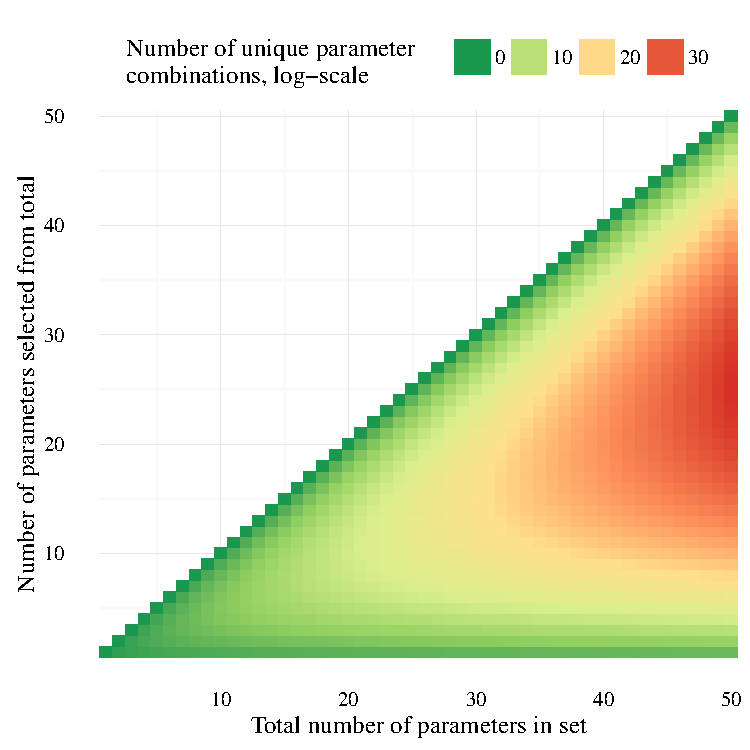
\includegraphics[width=0.6\textwidth]{figs/combnex-1} 

}

\caption[Examples of unique parameter combinations from different parameter sets and number of selected parameters]{Examples of unique parameter combinations from different parameter sets and number of selected parameters.  The number of combinations are shown for increasing numbers of selected parameters from the total in the set, where 50 parameter sets are shown each with one through 50 total parameters. Note that the number of unique combinations is shown as the natural-log.}\label{fig:combnex}
\end{figure}



% sensitivity example of top
\begin{figure}[!ht]

{\centering 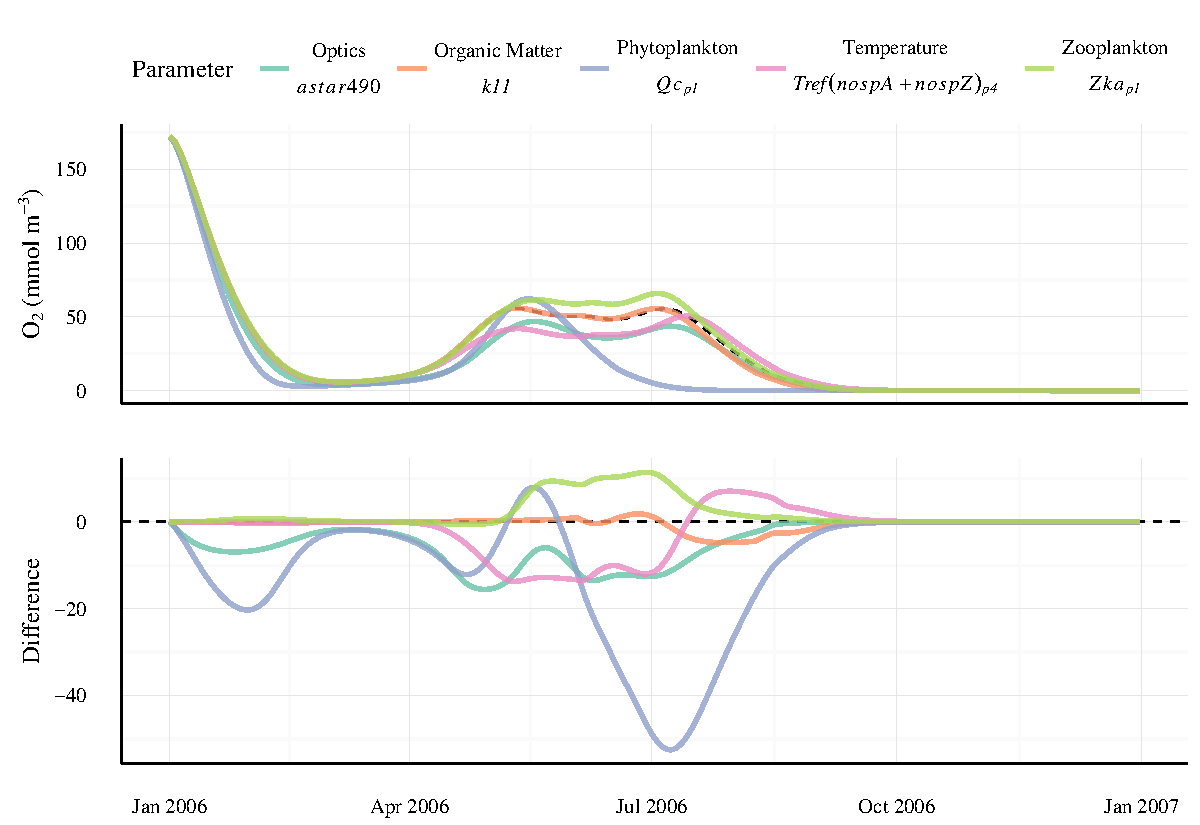
\includegraphics[width=\maxwidth]{figs/sensplo-1} 

}

\caption{Sensitivity of \ac{do} to parameter changes. The solid lines show the change in \ac{do} based on a 50\% change from the default parameter values (dashed line) for each parameter.  Individual parameters with the largest effect are shown for each category.  The top plot shows the model output and the middle plot shows the estimated \ac{do} as a difference from the default.  The bottom plot shows the distribution of error values (as $log\left(L1\right)$) for all parmaters in each category.}\label{fig:sensplo}
\end{figure}



% identifiability boxplots
\begin{figure}[!ht]

{\centering 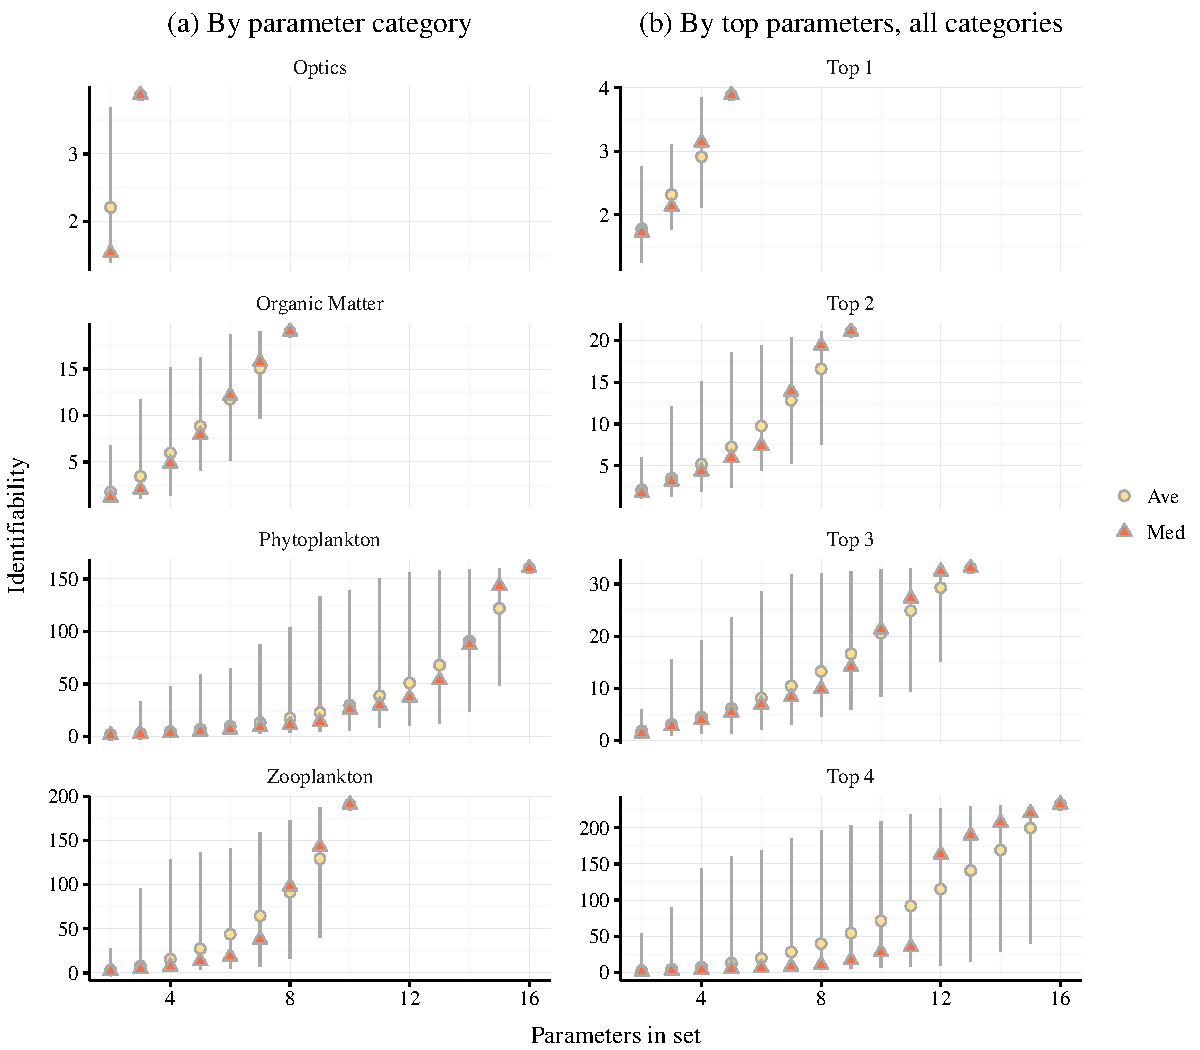
\includegraphics[width=\maxwidth]{figs/identbox-1} 

}

\caption[Identifiability (as ]{Identifiability (as $\gamma$, \cref{gameq}) of parameter subsets for \ac{do}.  Plots in (a) show identifiability by parameter categories and (b) shows identifiability by selecting the top 1 through 5 parameters regardless of category.  Lines represent identifiability ranges for the possible combinations given the number of parameters in the set.  The phytoplankton category is limited to 25 total parameters.}\label{fig:identbox}
\end{figure}



% parameter exclusion temp
\begin{figure}[!ht]

{\centering 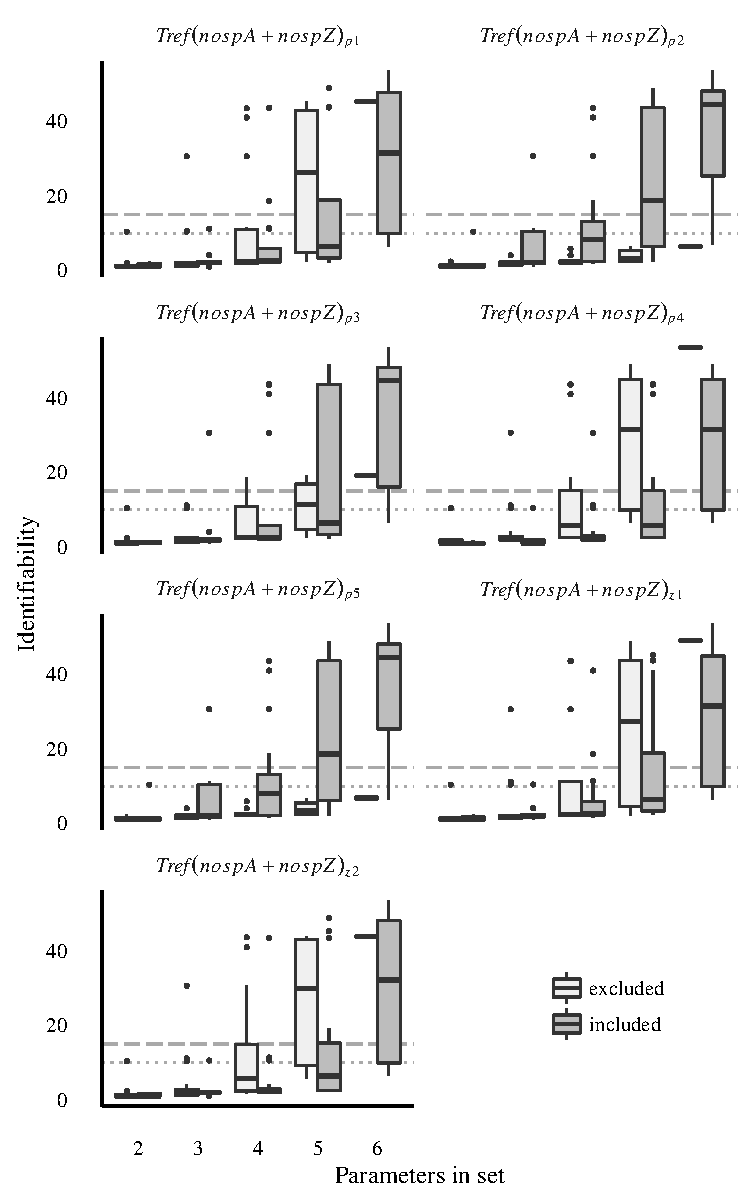
\includegraphics[width=0.6\textwidth]{figs/excltemp-1} 

}

\caption{Identifiability (as $\gamma$, \cref{gameq}) of temperature parameters for subset combinations in \cref{fig:identbox}.  Identifiability is evaluated for subsets that excluded and included the parameters at the top of each plot. Identifiability of including all seven parameters is in \cref{fig:identbox}. Grey lines indicate potential thresholds at $\gamma = 10, 15$ for maximum acceptable identifiability.}\label{fig:excltemp}
\end{figure}



% identifiability boxplot, p1, z1 only
\begin{figure}[!ht]

{\centering 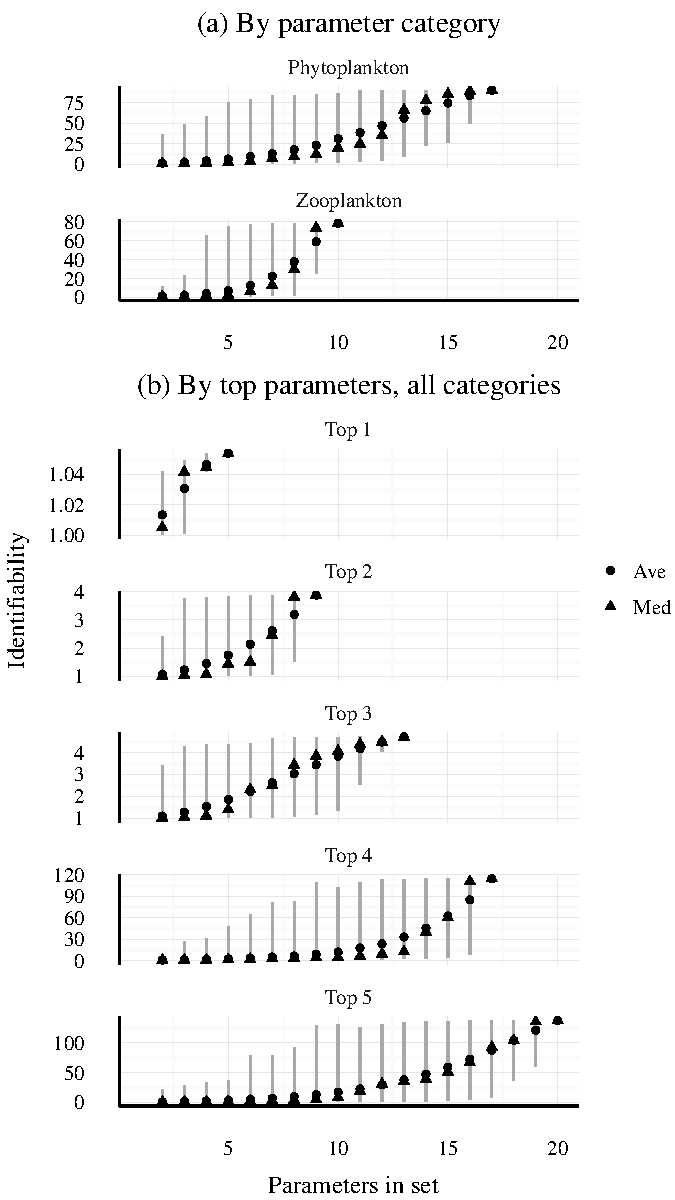
\includegraphics[width=0.5\textwidth]{figs/p1z1identbox-1} 

}

\caption[Identifiability (as ]{Identifiability (as $\gamma$, \cref{gameq}) of parameter subsets for \ac{do} using only subsets from the first phytoplankon group and first zooplankton group. Plots in (a) show identifiability for only the phytoplankton and zooplankton categories and (b) shows identifiability by selecting the top 1 through 5 parameters regardless of category. Lines represent identifiability ranges for the possible combinations given the number of parameters in the set.}\label{fig:p1z1identbox}
\end{figure}



% heuristic plots o2
\begin{figure}[!ht]

{\centering 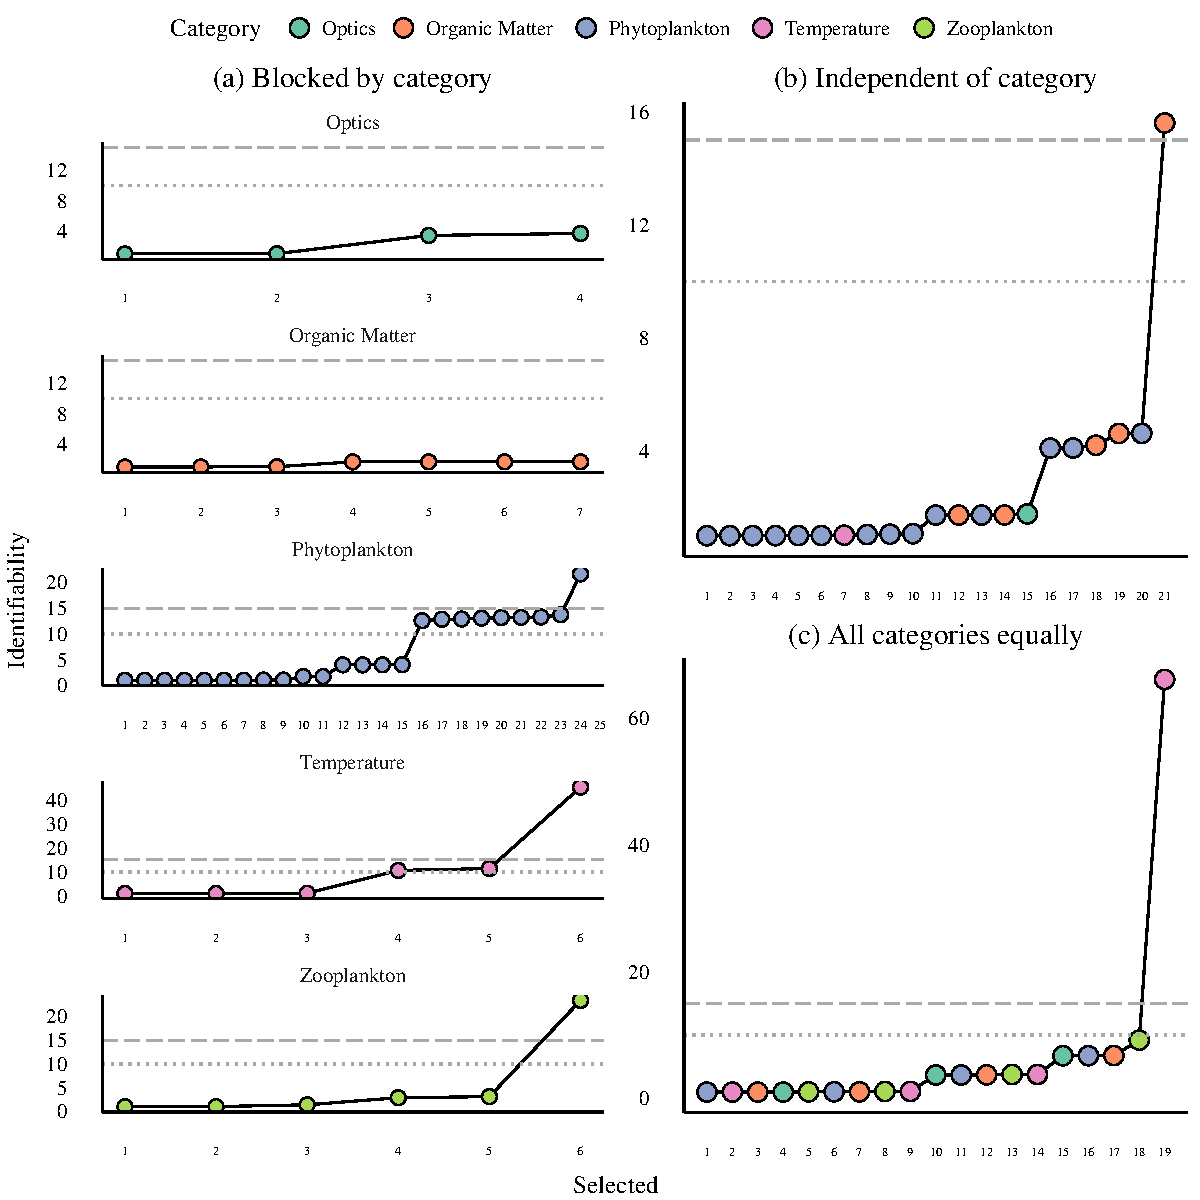
\includegraphics[width=\textwidth]{figs/heurist-1} 

}

\caption{Identifiability (as $\gamma$, \cref{gameq}) of selecting parameters with three different heuristics. Parameters are selected by decreasing sensitivity for all examples (\cref{tab:optsens,tab:tempsens,tab:phytosens,tab:zoopsens,tab:omsens}). The parameter selecions are blocked within each category (a), independent of category (b), or considering all categories equally (c). Grey lines indicate potential thresholds at $\gamma = 10, 15$ for maximum acceptable identifiability. Selection stops after $\gamma > 15$ or if the maximum number of possible parameters is selected.}\label{fig:heurist}
\end{figure}



% heuristic plots, all state
\begin{figure}[!ht]

{\centering 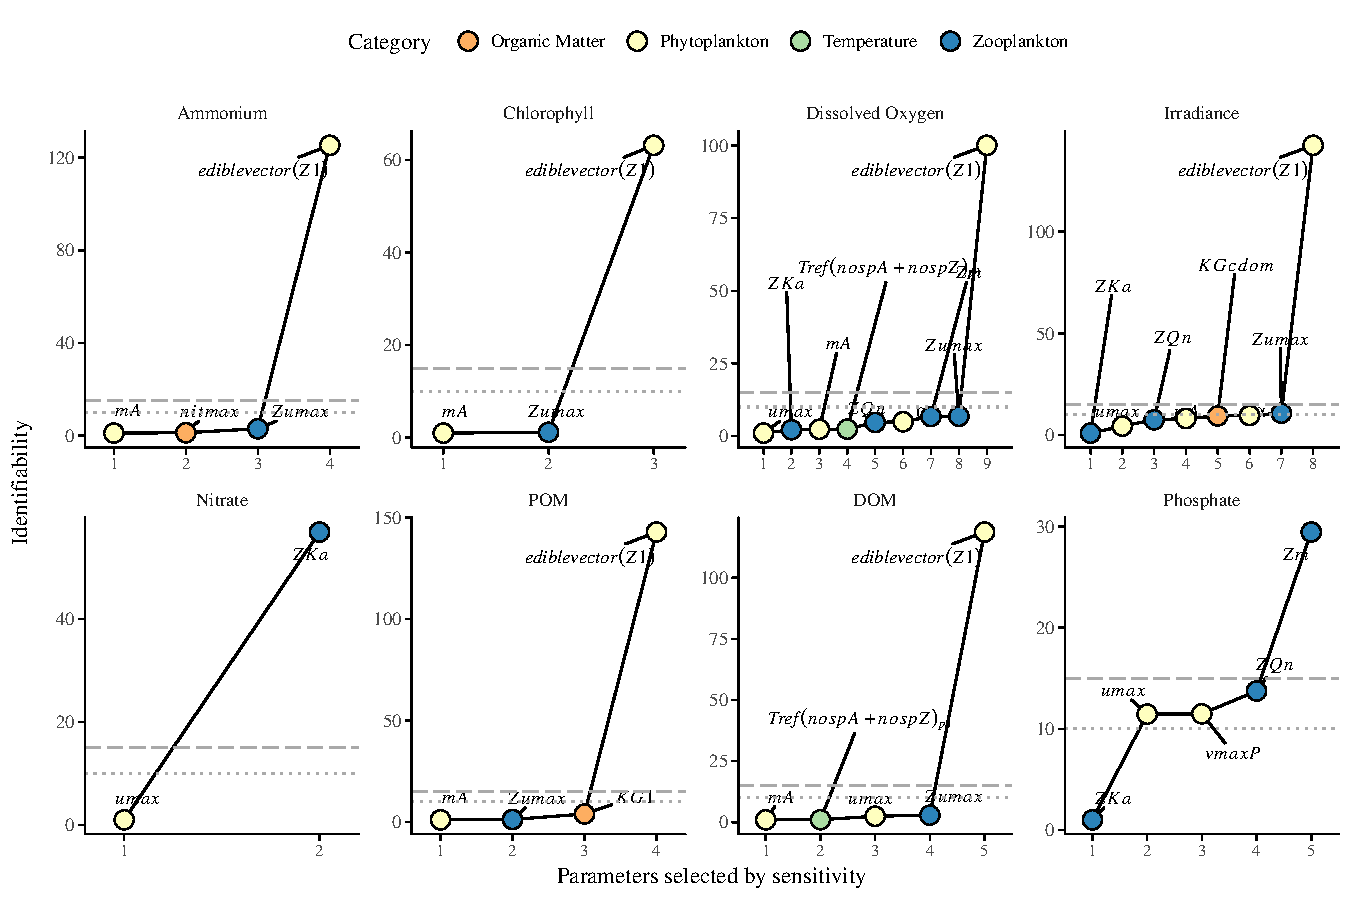
\includegraphics[width=\textwidth]{figs/heurist_stts-1} 

}

\caption[Identifiability (as ]{Identifiability (as $\gamma$, \cref{gameq}) of selecting parameters for selected state variables. Parameters are selected by decreasing sensitivity indepent of parameter categories. Grey lines indicate potential thresholds at $\gamma = 10, 15$ for maximum acceptable identifiability. Selection stops after $\gamma > 15$.}\label{fig:heurist_stts}
\end{figure}


\clearpage

% supplementary material
\beginsupplement

\begin{figure}[!ht]

{\centering 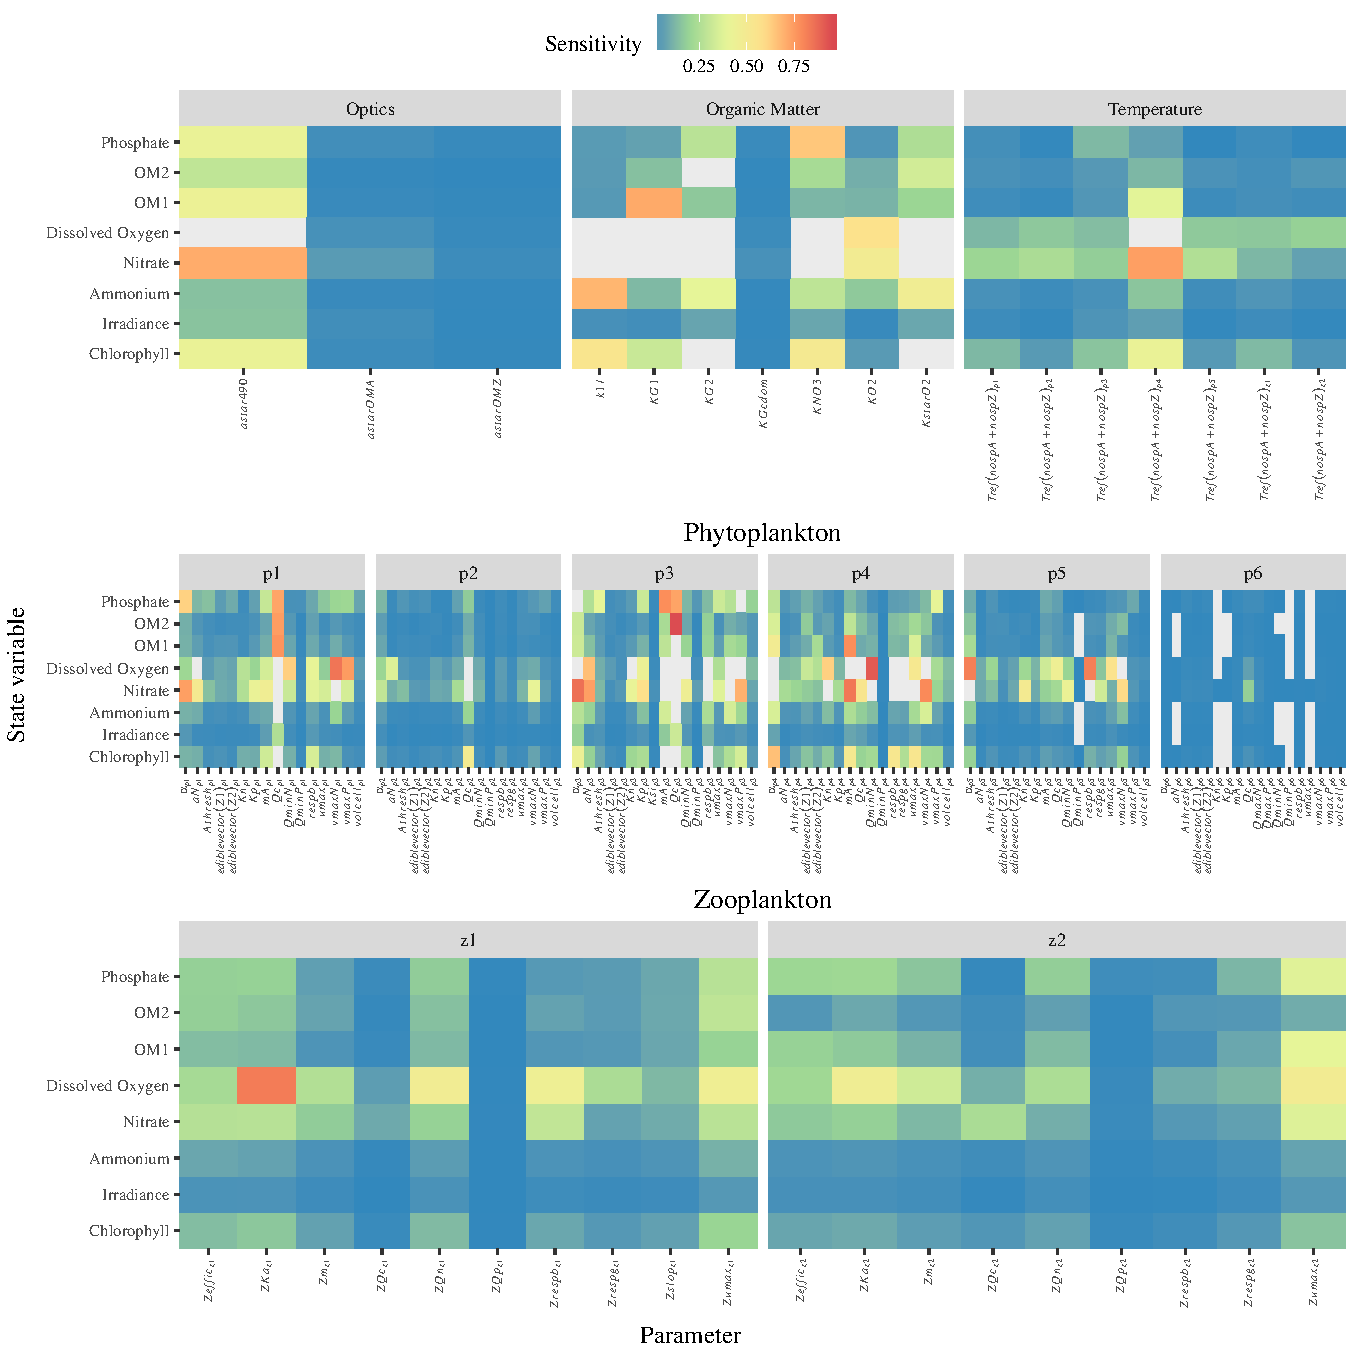
\includegraphics[width=\textwidth]{figs/sensalltile-1} 

}

\caption{Sensitivity values (L1, \cref{l1}) for local analyses of all state variables.  Values are truncated by the 5\textsuperscript{th} and 95\textsuperscript{th} sensitivity values between all parameters for visual appearance. Parameters are grouped by category (plot strips).  Phytoplankton and zooplankton categories are further separated into one through six, and one and two groups (p1-p6, z1, z2), respectively.}\label{fig:sensalltile}
\end{figure}




\end{document}
